\chapter{\emph{ATDlib}: A Library to Manage and Generate ATD}
\label{cha:atdlib}

This chapter presents \emph{ATDlib}, a reference implementation of the ATD
langauge described in Chapter~\ref{cha:atd} which implements parsing, automatic
generation and transformations of ATD. ATDlib is built using
\emph{Clojure}\cite{Hickey:2008:CPL:1408681.1408682}, which is compatible with
the Java virtual machine. An idiomatic Java wrapper is planned, but falls
outside the scope of this project. Section~\ref{sec:architecture} focuses on the
several tools provided in ATDlib and offers implementation details. Then,
Section~\ref{sec:atdlib_tour} shows an overview of the process of creating an
ATD from raw text data.

\section{Features and Architecture}
\label{sec:architecture}

The main goal behind ATDlib is to provide the necessary tooling in order to
support the implementation of ATD in organizations as a way of describing
business processes. This major goal can be split into the following
functionalities:


\begin{description}
  \item[Parsing and Representation of ATD]{ATD are stored as BRAT annotation
      files in \emph{standoff format}\cite{brat_standoff}. The standoff format
      is a text-based file that represents \emph{annotations} and
      \emph{relations} referencing a plain text file. Thus, an ATD will consist
      of a \texttt{Process.txt} with the textual description and a complementary
      \texttt{Process.ann} file with the annotations. ATDlib can parse this
      format and convert it to its internal schema, exposed in a public
      interface as shown in the UML diagram of Figure~\ref{fig:atdlib_uml}}
  \item[Automatic Annotation]{ATDlib can perform an initial annotation of a raw
      text in natural language. The goal is to perform the most accurate
      annotations possible. However, due to limitations in NLP, the annotations
      generated need to be reviewed by a human. Currently all annotation and
      relation types described in Section~\ref{sec:atd_semantics} are generated
      except the \emph{sequential}, \emph{exclusive} and \emph{parallel}
      relations, which must be manually annotated.}
  \item[Automatic Translation]{Several transformations are implemented for ATD
      in order to generate other process representations that interface with
      existing software. The goal is to establish ATD as a unique language for
      which any other representation can be automatically derived. These
      transformations can then be implemented as additional modules in ATDlib.
      Currently, the implemented transformations are to convert ATD into a
      FreeLing\cite{PadroS12} \emph{semantic graphs} and a \emph{behavioral
        profiles}\cite{smirnov2010business}}
    
\end{description}


ATDlib is structured as a single java library with several entry points,
corresponding to its different modules. Figure~\ref{fig:atdlib_architecture}
shows an overview of the different entry points, and their main functionalities.
The \texttt{brat\_parser} module is intended to be used as a library, and can be
used to read an annotation file into a more friendly format. The \texttt{text2atd}
entry point can be used as a standalone tool or as a library, and converts
textual descriptions into partially annotated ATD, which should then be checked
by a human using any compatible annotation tool, such as BRAT. Finally, the
\texttt{atd2fl} and \texttt{atd2bp} modules can be used as libraries to extract
a FreeLing semantic graph and a behavioral provile respectively. The inference
rules described in Section~\ref{sec:atd_reasoning} are applied during the
transformations. As mentioned in Section~\ref{sec:background_nlp4bpm}, the
semantic graph and the behavioral profiles can then be applied directly as input
data to the algorithms in the \emph{NLP4BPM} project.

\begin{figure}[htb]
  \centering
  \includegraphics[width=0.75\textwidth]{figures/atdlib_arch}
  \caption{ATDlib feature overview}
  \label{fig:atdlib_architecture}
\end{figure}


\begin{figure}[htb]
  \centering
  \includegraphics[width=\textwidth]{figures/atdlib_uml}
  \caption{UML diagram showing the public interface used for ATD representation}
  \label{fig:atdlib_uml}
\end{figure}

\subsection{Converting ATD to Freeling Semantic Graphs}

\todo{cross-reference this section above}

ATD and Freeling semantic graphs hold very similar information. Given the
graph-based nature of both representations, this conversion can be thought of as
a \emph{schema mapping} problem. However, some aspects need to be taken into
consideration to perform the conversion in a way that improves the quality of
the algorithms in the \emph{NLP4BPM} project, which is one the main application of
this library.

The conversion performed by the \texttt{atd2fl} module consists of
translating the concepts in ATD to a semantic graph, which consistis of the
following information:

\begin{itemize}
\item A list of \emph{entities}, which are nodes in the graph that correspond
  to the groups of connected components of \emph{entities} in the ATD when
  considering the \emph{coreference} relation. 
\item A list of \emph{frames}, nodes that correspond to \emph{action}
  annotations in the ATD
\item Relations between entities and frames. Currently supported are
  \emph{A0} (agent) and \emph{A1} (patient). However, some ATD expansions
  could map new relations such as the \emph{AM-MNR} (manner adjunct) or
  \emph{AM-LOC} (location adjunct).
\end{itemize}

But in order to have a complete textual representation for other tools to use,
the following information must also be extracted from an ATD:

\begin{itemize}
\item Lists of paragraphs, sentences and tokens
\item For each token \begin{itemize}
  \item The word's form and lemma.
  \item The part-of-speech (PoS) of the word.
  \item For nouns, verbs, adjectives and adverbs; a WordNet reference to the
    sense of the word.
  \end{itemize}
\end{itemize}

This information is necessary because FreeLing's semantic graph is expressed by
referencing certain words in the text, but including this information in
the ATD would require extensive unnecessary annotation, which doesn't align well
with the ATD's rationale. That is why \texttt{atd2fl} performs a low-level
analysis on the text (up to the sense disambiguation stage) using FreeLing to
automatically extract that information. This low-level information is then
merged with the ATD, in order to build a full semantic graph. During this
conversion, only the tokens that are part of some annotation in the ATD are kept
in the final structure, and all other words are removed.



\section{Creating an ATD with \emph{ATDlib}}
\label{sec:atdlib_tour}

Figure~\ref{fig:atdlib_process} illustrates the steps that must be taken in
order to generate a full ATD with ATDlib. First, a human actor must describe
the business process using natural language, creating a \texttt{MyProcess.txt}
file. Next, the \texttt{text2atd} module is used in order to obtain an
annotation file, \texttt{MyProcess.ann}. The user can then inspect the generated
annotation using the BRAT web interface. Figure~\ref{fig:brat_example} (left)
shows an example of what the user will see in the screen at this point. The user
must then refine the annotation, usually this process consists of deleting the
irrelevant actions detected by ATDlib, as well as marking the control flow for
the final set of actions, resulting in an annotation file similar to the one
shown in Figure~\ref{fig:brat_example} (right). Finally, if necessary, ATDlib
can be used to generate other process model representations, such as a FreeLing
semantic graph using the \texttt{atd2fl} module.

\begin{figure}[htb]
  \centering
  \begin{minipage}{0.49\textwidth}
  \includegraphics[width=\textwidth]{figures/ann_example_auto}
  \end{minipage}
  \begin{minipage}{0.49\textwidth}
  \includegraphics[width=\textwidth]{figures/ann_example_final}
  \end{minipage}
  \caption{The brat user interface: (left) An automatically generated
    ATD. (right) After the user performs a manual validation.}
  \label{fig:brat_example}
\end{figure}


\begin{figure}[htb]
  \centering
  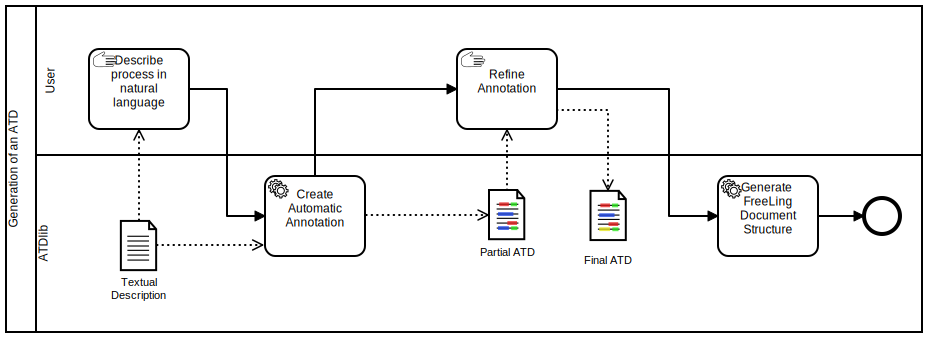
\includegraphics[width=\textwidth]{figures/atdlib_bpmn}
  \caption{Workflow of the creation of an ATD using ATDlib}
  \label{fig:atdlib_process}
\end{figure}

